
\section{Transforming Lattices into Matrices\label{sec:data-format}}
When training a NN on non purely numerical data, lattices in our case, it is necessary to first represent the data in a numerical form.
The choice of the data, as well as the quality of the representation, noticeably affect the quality of the resulting model.
Typically, a bad representation makes learning hard if not impossible, while a well-thought representation of the data is already half the job done.
Also, the model will perform better and be better at generalizing when trained on more and more varied data.
%The choice of the data representation and of the model architecture are dependent on each other. 

We decide to learn on randomly generated FCs and the corresponding lattices.
The main reason is that gathering and preparing large amounts of usable real-world FC is costly, while generating random data is cheap.
We can afford to use randomly generated FCs because we want to learn the general process of FCA, which should behave the same no matter the source of the data.

In this section, we describe the lattice data we used for our experiments and how we encode it as matrices.
First, we explain our generation process in \cref{sec:data-generation}.
We then explain how we adapted the breadth-first search ordering method of GraphRNN in \cref{sec:level-order}.
We then discuss the encoding of the adjacency in \cref{sec:enc-adjacency} and the intents and extents in \cref{sec:enc-intents-extents}.

\subsection{Data Generation and Dataset\label{sec:data-generation}}
The dataset used for training the GraphRNN models is composed of 4000 randomly generated FCs and the corresponding lattices computed using the Coron system\footnote{\url{http://coron.loria.fr/site/index.php}}.
To generate a context of $|O|$ objects and $|A|$ attributes we sample $|O|\times|A|$ values from a Poisson distribution and apply a threshold of $0.3$.
The values under this threshold correspond to $1$ in the context, which leads to a density (the portion of entries equal to $1$) around $0.3$.
Note that the random generation process may result in empty rows and columns, which will be dropped by Coron if they are at the extremities of the context.
For this reason, the actual size of the generated context may be smaller than the requested one.
For the training phase, a development set of 10\% of the training set is randomly sampled from the training set. 
We generate different sizes of contexts: 2000 of $5 \times 5$, 1000 of $10 \times 10$, 500 of $10 \times 20$, and 500 of $20 \times 10$ ($|O|\times|A|$).
The statistics of the generated dataset are reported in \cref{tab:rand-dataset-1}.
The dataset itself and the generation process are available in a GitLab repository\footnote{\url{https://gitlab.inria.fr/emarquer/random-lattice-dataset}}.

%We also use a smaller dataset of 6 FCs and lattices of less than 5 objects and attributes for basic qualitative experiments.

\begin{table}[t]
\centering
\begin{tabularx}{\textwidth}{rr>{\raggedleft\arraybackslash}X>{\raggedleft\arraybackslash}X>{\raggedleft\arraybackslash}X}
\toprule
 &  &  & \multicolumn{2}{r}{Density of the triangular adjacency} \\
 & Size & \# Concept & Graph of $\prec$ & Graph of $\leq$ \\
\midrule
\multirow{5}{*}{Mean $\pm$~std.}
& All            & $27.35 \pm 24.76$ & $0.12 \pm 0.07$ & $0.22 \pm 0.09$ \\
& $5 \times 5$   & $7.28 \pm 1.88$ & $0.18 \pm 0.02$ & $0.30 \pm 0.03$ \\
& $10 \times 10$ & $29.49 \pm 6.30$ & $0.07 \pm 0.01$ & $0.17 \pm 0.02$ \\
& $10 \times 20$ & $66.00 \pm 11.55$ & $0.038 \pm 0.005$ & $0.11 \pm 0.01$ \\
& $20 \times 10$ & $64.68 \pm 13.05$ & $0.039 \pm 0.006$ & $0.11 \pm 0.01$ \\
\midrule
\multirow{5}{*}{Range}
& All & 1 to 117 & 0 to 0.25 & 0 to 0.39 \\
& $5 \times 5$   & 1 to 15 & 0 to 0.25 & 0 to 0.39 \\
& $10 \times 10$ & 15 to 64 & 0.04 to 0.11 & 0.12 to 0.29 \\
& $10 \times 20$ & 38 to 114 & 0.025 to 0.054 & 0.08 to 0.15 \\
& $20 \times 10$ & 37 to 117 & 0.024 to 0.058 & 0.08 to 0.16 \\
\bottomrule
\end{tabularx}
\caption{Descriptive statistics on the dataset of randomly generated contexts.}\label{tab:rand-dataset-1}
\end{table}

\subsection{From Breath-First Search to Level Ordering\label{sec:level-order}}
In GraphRNN~\cite{graphrnn:2018:jiaxuan}, a graph is represented by its adjacency.
The graph is flattened into a sequence with a \textit{breadth-first search} (BFS), each element of the sequence describing a node by defining its adjacency with the previous nodes in the sequence.
In practice, we have a sequence $S^\pi = (S^\pi_1, \dots, S^\pi_n)$ for a graph of $n$ nodes ordered by $\pi$, with $S^\pi_i \in \{0, 1\}^{i-1}$ an adjacency vector for the node $i$ with the nodes $1$ to  $i-1$.
The breadth-first search order $\pi$ ensures that the distance between the two adjacent nodes in the sequence is small, as demonstrated in~\cite{graphrnn:2018:jiaxuan}.
This method is designed for undirected graphs but also works for directed graphs, under the condition of using $S^\pi_i \in \{-1, 0, 1\}^{i-1}$ to represent both incoming and outgoing edges.

We adapt the methodology of~\cite{graphrnn:2018:jiaxuan} to lattices by defining an ordering of concepts based on what we call \textit{levels}.
First, we define levels in \cref{def:level}.
\begin{definition}\label{def:level}
We iteratively define $L$, the indexed set of levels and a partition of $C$, such as %$L\in\mathcal{L}$ $L\in 2^C$
%We designate levels by an index in $\mathds{N}$.
a concept $c_1 \in C$ belongs to the \textit{level} $l_i\in L$ if and only if the highest level of every other concept $c_2 \in C, c_2 \prec c_1$
belongs to  is $i-1$.
\end{definition}
For a given lattice, $L$ can be demonstrated to be unique.
Due to the way levels are defined, two concepts within the same level are not comparable with the partial order $\leq$.
Additionally, if a concept $c_1$ belongs to a lower level than a concept $c_2$, either $c_1$ and $c_2$ are not comparable or $c_2 \leq c_1$.
Finally, $\bot$ is the only concept in level $0$ and $\top$ is the only concept in the highest level.
%
We can now define the \textit{level-based order} $\mathcal{O}^L = (c_0, \dots, c_n)$ an ordering of $C$ based on $L$.
%$\mathcal{O}^L_i$ the such as
This order is constructed by concatenating the levels from $l_0$ to $l_{|L|}$.
The order of the concepts within each level does not matter and is thus arbitrarily chosen.
The levels of the example from \cref{fig:hasse} and the corresponding level-based order are shown in \cref{fig:level-order}.

\begin{figure}
    \centering
    %\includegraphics{}
    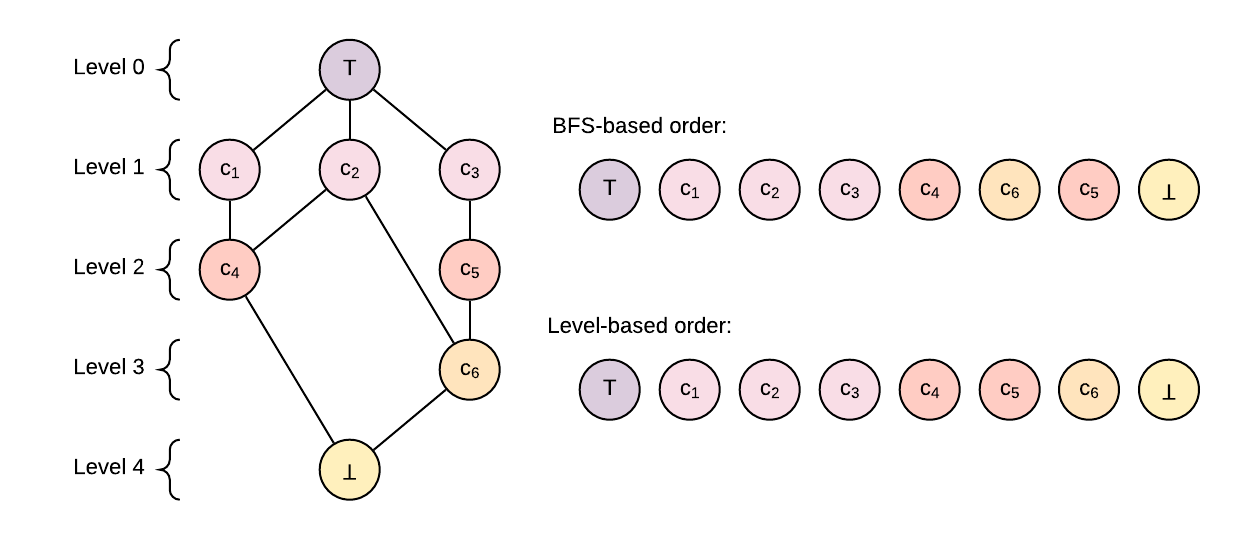
\includegraphics[keepaspectratio, width=.9\textwidth, height=5cm]{Figures/Ch1/example_order.png}
    \caption{Lattice from \cref{fig:hasse} organized in levels and the corresponding level-based and BFS-based orders.}
    \label{fig:level-order}
\end{figure}

Using this new order $\mathcal{O}^L$ with the method of~\cite{graphrnn:2018:jiaxuan} maintains most of the properties demonstrated in~\cite{graphrnn:2018:jiaxuan}.
However, the distance between related nodes (concepts in our case) is less constrained, as concepts of the last layers can be related by $\prec$ with concepts of first layers.
%In practice, this distance between related nodes does not
Conversely, using level-based ordering instead of BFS allows the adjacency vectors to contain only outgoing edges and no incoming ones.
Indeed, for all $c_1, c_2 \in C$ such that $c_1 \prec c_2$, if $c_1 \in l_i$ then $c_2 \in l_j$ with $i < j$.
In other words, a concept is only related to previous elements in the order.

In our example, BFS and level-based ordering produce different results.
Indeed, $c_6$ appears before $c_5$ with BFS, so we need to represent the relation of $c_6$ and $c_5$ with an incoming edge from $c_6$ in the adjacency list of $c_5$.
However, in the level-based ordering $c_6$ appears after $c_5$ and there is no need for incoming edges.

\subsection{Encoding the Lattice Adjacency\label{sec:enc-adjacency}}
%\todo[inline]{The whole subsection is a work in progress}
The lattice adjacency can be encoded in multiple ways.
A first method is to directly consider the sequence of adjacency vectors of different sizes as in~\cite{graphrnn:2018:jiaxuan}.
A second method consists in concatenating the adjacency vectors, and a third method is to use the adjacency matrix as described in the following paragraph.
For practical purposes, we tend to represent the data as vectors or matrices, so we focus on the last two representations.
The concatenation of the adjacency vectors is the most optimal in terms of used space, while the adjacency matrix separates the adjacency of each node across one of the dimensions. The adjacency matrix provides additional benefits, like an easier visualization and simpler manipulation of the adjacency. However, the adjacency matrix requires twice the space of the concatenated adjacency vectors, as the upper triangular matrix is not used.

\subsubsection{Basic Adjacency Matrix}
We define a matrix $\mathbf{L}$ such that the entry at row $i$ and column $j$, $\mathbf{L}_{i,j} = S^{\mathcal{O}L}_{i,j}$, with $S^{\mathcal{O}L}_{i,j}$ the element at position $j$ in $S^{\mathcal{O}L}_i$.
Where $S^{\mathcal{O}L}_{i,j}$ is not defined ($i \leq j$), $\mathbf{L}_{i,j} = 0$.
In other words, we fill a lower triangular matrix with the adjacency vectors.
The resulting lower triangular matrix is the adjacency matrix in the case of $\prec$ and $<$.
For $\leq$, the diagonal ($i = j$) of the matrix of $<$ must be set to 1.

When using a model to predict this matrix, we are in a binary classification problem between two classes: NO EDGE ($0$) and EDGE ($1$).
The model can thus be trained using BCE.

\subsubsection{Adjacency Matrix \emph{à la} Sequence Modeling}
GraphRNN is an architecture designed to process a sequence of nodes, each represented by a sequence of edges.
Traditionally when using RNNs to process sequences we use special values to mark boundaries in the sequence, \eg, the start and end of the sequence.
A special value is also dedicated to padding the sequence. This padding value is used to make the sequence of a batch have the same size.

We also propose to make use of the empty space in the upper triangular matrix.
The transpose of the adjacency matrices of $\prec$, $<$, and $\leq$ are respectively the adjacency matrices of $\succ$, $>$, and $\geq$.
For our triangular matrix containing only outgoing edges from the nodes, the transposed matrix represents the incoming edges.
This transposed matrix is upper triangular, and we use it to fill the unused space of the lower triangular matrix.
Using this construction, we have redundancy between the lower and upper triangular matrices.
This redundancy can prove beneficial for our task, as we can use the upper triangular matrix to check the results of the lower one.

For each node of the graph, we have a sequence of values as follows:
\begin{enumerate}
    \item a \textit{start of sequence} (SOS) value;
    \item the sequence of outgoing edges, either $1$ if there is an edge or $0$ otherwise;
    \item a \textit{middle of sequence} (MOS) value;
    \item the sequence of incoming edges, either $1$ if there is an edge or $0$ otherwise;
    \item an \textit{end of sequence} (EOS) value;
    \item as many \textit{padding} (PAD) values as necessary to reach the size of the largest element in the batch.
\end{enumerate}
We also add sequences full of PAD in the sequence of nodes to reach the size of the largest element in the batch.
The resulting data takes the form of a matrix containing one of 6 values in each entry: NO EDGE ($0$), EDGE ($1$), SOS, MOS, EOS, and PAD.
An example of a batch encoded using this process is shown in \cref{fig:data-pad}.

\begin{figure}
    \centering
    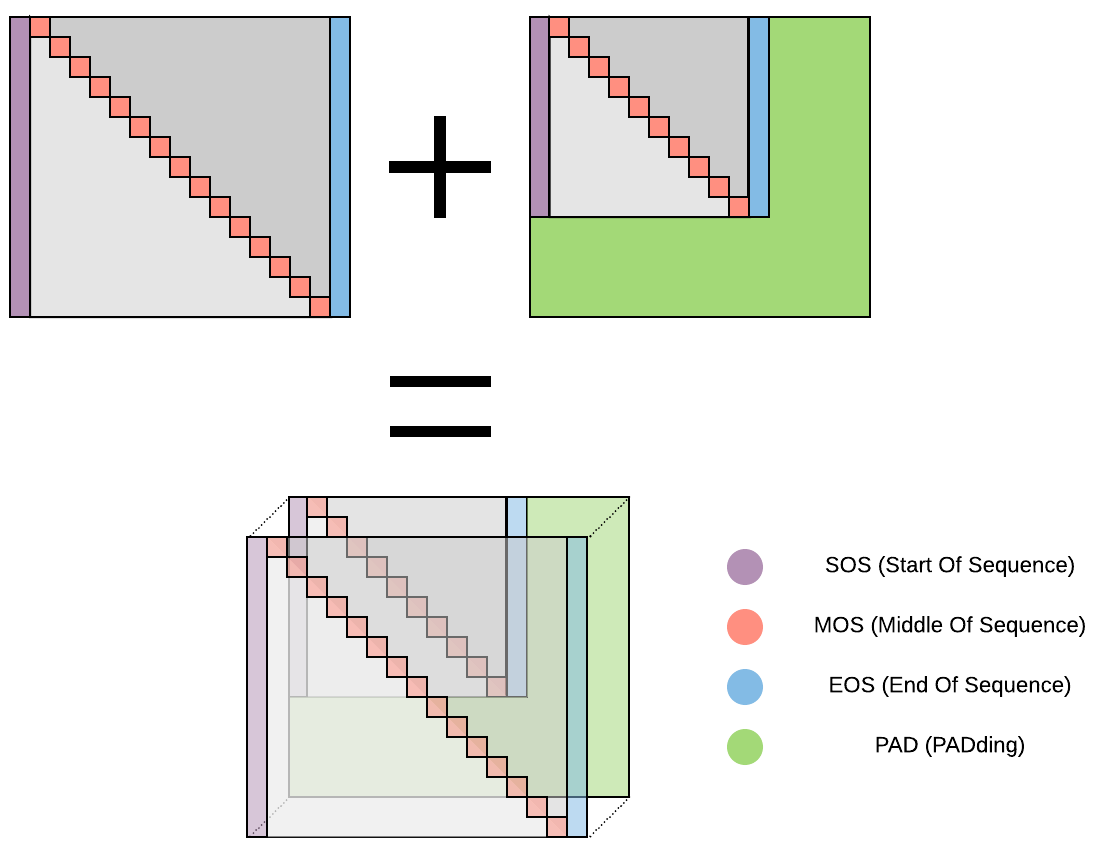
\includegraphics[keepaspectratio, width=.9\textwidth, height=10cm]{Figures/Ch1/pad.png}
    \caption{Diagram of a batch of 2 samples encoded using the 6 values NO EDGE ($0$) and EDGE ($1$) for the adjacency, SOS, MOS, EOS, and PAD.}
    \label{fig:data-pad}
\end{figure}

When using a model to predict this matrix, we are in a multi-label classification problem between 6 classes corresponding to the possible values.
The model can thus be trained using cross-entropy.

\subsection{Encoding the Concepts\label{sec:enc-intents-extents}}
Concepts can be represented using either their intents, their extents, or both.
In FCA, there are two ways to encode the intents and the extents: the \textit{full encoding} and the \textit{narrow encoding}.
Using the full encoding, all the attributes (or objects) of the intent (respectively extent) are used to represent a concept.
The narrow encoding however only use the attributes (or object) that ``appear'' in the concept, in other words, the attributes (respectively objects) that are present in the concept's intent (respectively extent) but not in the ones lower (respectively higher) according to the partial order $\leq$.
To reconstruct the full intent (respectively extent) of a concept from the narrow encoding, we take the set of all the attributes (respectively objects) in the narrow encoding of the concept and the ones of concepts lower (respectively higher) according to $\leq$.
An interesting property of this narrow representation is that each attribute (and object) appear only once in the lattice.
\cref{fig:encoding} shows the narrow encoding of the example lattice from \cref{fig:hasse}.

\begin{figure}
    \centering
    %\includegraphics{}
    %\subcaptionbox{Full encoding ()}{
    %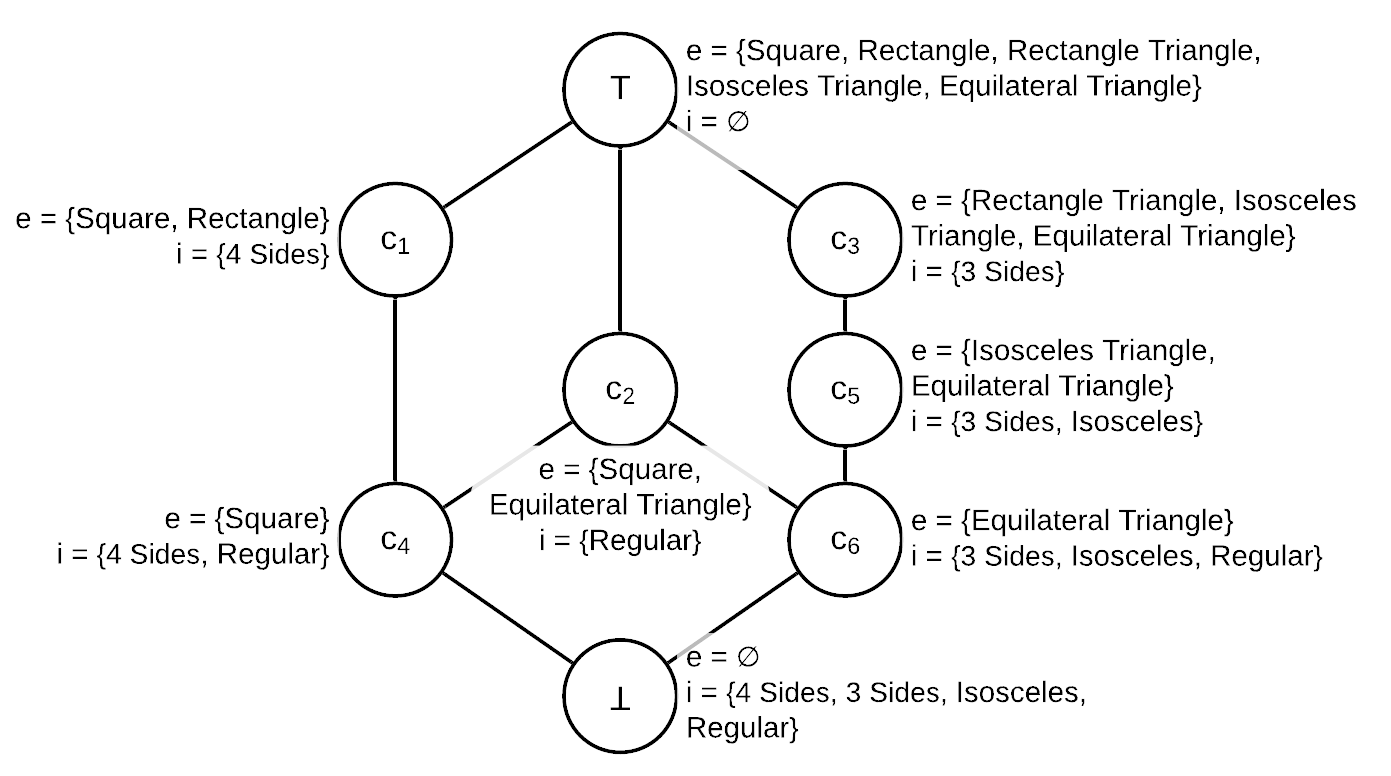
\includegraphics[keepaspectratio, height=8cm, width=.56\textwidth]{Figures/Ch0/example_full.png}}
    %\subcaptionbox{Narrow encoding}{
    %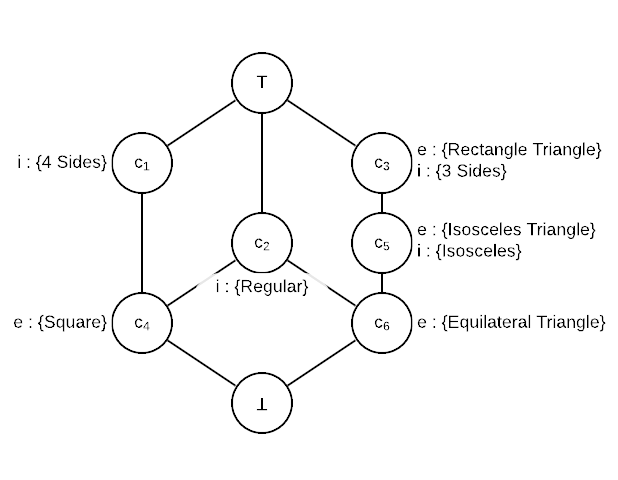
\includegraphics[keepaspectratio, height=8cm, width=.42\textwidth]{Figures/Ch0/example_narrow.png}}
    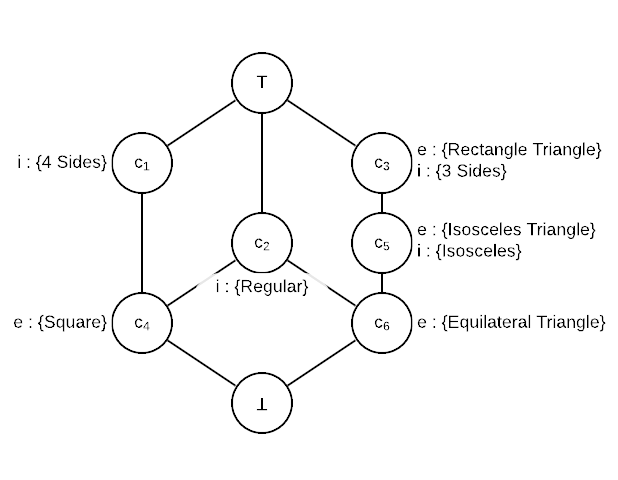
\includegraphics[keepaspectratio, height=7cm, width=.9\textwidth]{Figures/Ch0/example_narrow.png}
    \caption{Narrow encoding of the example lattice of \cref{fig:hasse}.}
    \label{fig:encoding}
\end{figure}

We design two numerical representations for the concepts.
The first one is a matrix based on the full encoding.
The entry at row $i$ and column $j$ is $1$ if the attribute $a_j$ (or object $o_j$) is present in the intent (respectively extent) of the concept indexed $i$ in $\mathcal{O}^L$, and $0$ otherwise.
The second representation is based on the narrow encoding. It takes the form of a vector, with each entry corresponding to an attribute (or object).
The value of an entry is the index in $\mathcal{O}^L$ in which the corresponding attribute (respectively object) ``appears''.


